\documentclass[twoside]{book}

% Packages required by doxygen
\usepackage{fixltx2e}
\usepackage{calc}
\usepackage{doxygen}
\usepackage[export]{adjustbox} % also loads graphicx
\usepackage{graphicx}
\usepackage[utf8]{inputenc}
\usepackage{makeidx}
\usepackage{multicol}
\usepackage{multirow}
\PassOptionsToPackage{warn}{textcomp}
\usepackage{textcomp}
\usepackage[nointegrals]{wasysym}
\usepackage[table]{xcolor}

% Font selection
\usepackage[T1]{fontenc}
\usepackage[scaled=.90]{helvet}
\usepackage{courier}
\usepackage{amssymb}
\usepackage{sectsty}
\renewcommand{\familydefault}{\sfdefault}
\allsectionsfont{%
  \fontseries{bc}\selectfont%
  \color{darkgray}%
}
\renewcommand{\DoxyLabelFont}{%
  \fontseries{bc}\selectfont%
  \color{darkgray}%
}
\newcommand{\+}{\discretionary{\mbox{\scriptsize$\hookleftarrow$}}{}{}}

% Page & text layout
\usepackage{geometry}
\geometry{%
  a4paper,%
  top=2.5cm,%
  bottom=2.5cm,%
  left=2.5cm,%
  right=2.5cm%
}
\tolerance=750
\hfuzz=15pt
\hbadness=750
\setlength{\emergencystretch}{15pt}
\setlength{\parindent}{0cm}
\setlength{\parskip}{3ex plus 2ex minus 2ex}
\makeatletter
\renewcommand{\paragraph}{%
  \@startsection{paragraph}{4}{0ex}{-1.0ex}{1.0ex}{%
    \normalfont\normalsize\bfseries\SS@parafont%
  }%
}
\renewcommand{\subparagraph}{%
  \@startsection{subparagraph}{5}{0ex}{-1.0ex}{1.0ex}{%
    \normalfont\normalsize\bfseries\SS@subparafont%
  }%
}
\makeatother

% Headers & footers
\usepackage{fancyhdr}
\pagestyle{fancyplain}
\fancyhead[LE]{\fancyplain{}{\bfseries\thepage}}
\fancyhead[CE]{\fancyplain{}{}}
\fancyhead[RE]{\fancyplain{}{\bfseries\leftmark}}
\fancyhead[LO]{\fancyplain{}{\bfseries\rightmark}}
\fancyhead[CO]{\fancyplain{}{}}
\fancyhead[RO]{\fancyplain{}{\bfseries\thepage}}
\fancyfoot[LE]{\fancyplain{}{}}
\fancyfoot[CE]{\fancyplain{}{}}
\fancyfoot[RE]{\fancyplain{}{\bfseries\scriptsize Generated by Doxygen }}
\fancyfoot[LO]{\fancyplain{}{\bfseries\scriptsize Generated by Doxygen }}
\fancyfoot[CO]{\fancyplain{}{}}
\fancyfoot[RO]{\fancyplain{}{}}
\renewcommand{\footrulewidth}{0.4pt}
\renewcommand{\chaptermark}[1]{%
  \markboth{#1}{}%
}
\renewcommand{\sectionmark}[1]{%
  \markright{\thesection\ #1}%
}

% Indices & bibliography
\usepackage{natbib}
\usepackage[titles]{tocloft}
\setcounter{tocdepth}{3}
\setcounter{secnumdepth}{5}
\makeindex

% Hyperlinks (required, but should be loaded last)
\usepackage{ifpdf}
\ifpdf
  \usepackage[pdftex,pagebackref=true]{hyperref}
\else
  \usepackage[ps2pdf,pagebackref=true]{hyperref}
\fi
\hypersetup{%
  colorlinks=true,%
  linkcolor=blue,%
  citecolor=blue,%
  unicode%
}

% Custom commands
\newcommand{\clearemptydoublepage}{%
  \newpage{\pagestyle{empty}\cleardoublepage}%
}

\usepackage{caption}
\captionsetup{labelsep=space,justification=centering,font={bf},singlelinecheck=off,skip=4pt,position=top}

%===== C O N T E N T S =====

\begin{document}

% Titlepage & ToC
\hypersetup{pageanchor=false,
             bookmarksnumbered=true,
             pdfencoding=unicode
            }
\pagenumbering{alph}
\begin{titlepage}
\vspace*{7cm}
\begin{center}%
{\Large My Project }\\
\vspace*{1cm}
{\large Generated by Doxygen 1.8.13}\\
\end{center}
\end{titlepage}
\clearemptydoublepage
\pagenumbering{roman}
\tableofcontents
\clearemptydoublepage
\pagenumbering{arabic}
\hypersetup{pageanchor=true}

%--- Begin generated contents ---
\chapter{Namespace Index}
\section{Namespace List}
Here is a list of all namespaces with brief descriptions\+:\begin{DoxyCompactList}
\item\contentsline{section}{\hyperlink{namespace_david_fricker}{David\+Fricker} }{\pageref{namespace_david_fricker}}{}
\item\contentsline{section}{\hyperlink{namespace_david_fricker_1_1_data_abstracter}{David\+Fricker\textbackslash{}\+Data\+Abstracter} }{\pageref{namespace_david_fricker_1_1_data_abstracter}}{}
\end{DoxyCompactList}

\chapter{Hierarchical Index}
\section{Class Hierarchy}
This inheritance list is sorted roughly, but not completely, alphabetically\+:\begin{DoxyCompactList}
\item \contentsline{section}{Content\+Contract}{\pageref{class_david_fricker_1_1_data_abstracter_1_1_content_contract}}{}
\item \contentsline{section}{Interface\+Content\+Provider}{\pageref{interface_david_fricker_1_1_data_abstracter_1_1_interface_content_provider}}{}
\begin{DoxyCompactList}
\item \contentsline{section}{Content\+Provider}{\pageref{class_david_fricker_1_1_data_abstracter_1_1_content_provider}}{}
\end{DoxyCompactList}
\item \contentsline{section}{Interface\+Database\+Wrapper}{\pageref{interface_david_fricker_1_1_data_abstracter_1_1_interface_database_wrapper}}{}
\begin{DoxyCompactList}
\item \contentsline{section}{My\+S\+Q\+L\+Database\+Wrapper}{\pageref{class_david_fricker_1_1_data_abstracter_1_1_my_s_q_l_database_wrapper}}{}
\end{DoxyCompactList}
\item P\+DO\begin{DoxyCompactList}
\item \contentsline{section}{My\+S\+Q\+L\+Database\+Wrapper}{\pageref{class_david_fricker_1_1_data_abstracter_1_1_my_s_q_l_database_wrapper}}{}
\end{DoxyCompactList}
\end{DoxyCompactList}

\chapter{Data Structure Index}
\section{Data Structures}
Here are the data structures with brief descriptions\+:\begin{DoxyCompactList}
\item\contentsline{section}{\hyperlink{class_david_fricker_1_1_data_abstracter_1_1_content_contract}{Content\+Contract} }{\pageref{class_david_fricker_1_1_data_abstracter_1_1_content_contract}}{}
\item\contentsline{section}{\hyperlink{class_david_fricker_1_1_data_abstracter_1_1_content_provider}{Content\+Provider} }{\pageref{class_david_fricker_1_1_data_abstracter_1_1_content_provider}}{}
\item\contentsline{section}{\hyperlink{interface_david_fricker_1_1_data_abstracter_1_1_interface_content_provider}{Interface\+Content\+Provider} }{\pageref{interface_david_fricker_1_1_data_abstracter_1_1_interface_content_provider}}{}
\item\contentsline{section}{\hyperlink{interface_david_fricker_1_1_data_abstracter_1_1_interface_database_wrapper}{Interface\+Database\+Wrapper} }{\pageref{interface_david_fricker_1_1_data_abstracter_1_1_interface_database_wrapper}}{}
\item\contentsline{section}{\hyperlink{class_david_fricker_1_1_data_abstracter_1_1_my_s_q_l_database_wrapper}{My\+S\+Q\+L\+Database\+Wrapper} }{\pageref{class_david_fricker_1_1_data_abstracter_1_1_my_s_q_l_database_wrapper}}{}
\end{DoxyCompactList}

\chapter{File Index}
\section{File List}
Here is a list of all files with brief descriptions\+:\begin{DoxyCompactList}
\item\contentsline{section}{D\+:/\+X\+A\+M\+P\+P/htdocs/\+Data\+Abstracter/src/\hyperlink{_content_contract_8php}{Content\+Contract.\+php} }{\pageref{_content_contract_8php}}{}
\item\contentsline{section}{D\+:/\+X\+A\+M\+P\+P/htdocs/\+Data\+Abstracter/src/\hyperlink{_content_provider_8php}{Content\+Provider.\+php} }{\pageref{_content_provider_8php}}{}
\item\contentsline{section}{D\+:/\+X\+A\+M\+P\+P/htdocs/\+Data\+Abstracter/src/\hyperlink{_interface_content_provider_8php}{Interface\+Content\+Provider.\+php} }{\pageref{_interface_content_provider_8php}}{}
\item\contentsline{section}{D\+:/\+X\+A\+M\+P\+P/htdocs/\+Data\+Abstracter/src/\hyperlink{_interface_database_wrapper_8php}{Interface\+Database\+Wrapper.\+php} }{\pageref{_interface_database_wrapper_8php}}{}
\item\contentsline{section}{D\+:/\+X\+A\+M\+P\+P/htdocs/\+Data\+Abstracter/src/\hyperlink{_my_s_q_l_database_wrapper_8php}{My\+S\+Q\+L\+Database\+Wrapper.\+php} }{\pageref{_my_s_q_l_database_wrapper_8php}}{}
\item\contentsline{section}{D\+:/\+X\+A\+M\+P\+P/htdocs/\+Data\+Abstracter/src/\hyperlink{test_8php}{test.\+php} }{\pageref{test_8php}}{}
\end{DoxyCompactList}

\chapter{Namespace Documentation}
\hypertarget{namespace_david_fricker}{}\section{David\+Fricker Namespace Reference}
\label{namespace_david_fricker}\index{David\+Fricker@{David\+Fricker}}
\subsection*{Namespaces}
\begin{DoxyCompactItemize}
\item 
 \hyperlink{namespace_david_fricker_1_1_data_abstracter}{Data\+Abstracter}
\end{DoxyCompactItemize}

\hypertarget{namespace_david_fricker_1_1_data_abstracter}{}\section{David\+Fricker\textbackslash{}Data\+Abstracter Namespace Reference}
\label{namespace_david_fricker_1_1_data_abstracter}\index{David\+Fricker\textbackslash{}\+Data\+Abstracter@{David\+Fricker\textbackslash{}\+Data\+Abstracter}}
\subsection*{Data Structures}
\begin{DoxyCompactItemize}
\item 
class \hyperlink{class_david_fricker_1_1_data_abstracter_1_1_content_contract}{Content\+Contract}
\item 
class \hyperlink{class_david_fricker_1_1_data_abstracter_1_1_content_provider}{Content\+Provider}
\item 
interface \hyperlink{interface_david_fricker_1_1_data_abstracter_1_1_interface_content_provider}{Interface\+Content\+Provider}
\item 
interface \hyperlink{interface_david_fricker_1_1_data_abstracter_1_1_interface_database_wrapper}{Interface\+Database\+Wrapper}
\item 
class \hyperlink{class_david_fricker_1_1_data_abstracter_1_1_my_s_q_l_database_wrapper}{My\+S\+Q\+L\+Database\+Wrapper}
\end{DoxyCompactItemize}

\chapter{Data Structure Documentation}
\hypertarget{class_david_fricker_1_1_data_abstracter_1_1_content_contract}{}\section{Content\+Contract Class Reference}
\label{class_david_fricker_1_1_data_abstracter_1_1_content_contract}\index{Content\+Contract@{Content\+Contract}}
\subsection*{Data Fields}
\begin{DoxyCompactItemize}
\item 
const \hyperlink{class_david_fricker_1_1_data_abstracter_1_1_content_contract_a20710e1b8d4d68cda1a9e322388eaa40}{D\+A\+T\+A\+\_\+\+T\+Y\+P\+E\+\_\+\+I\+NT} = \textquotesingle{}int\textquotesingle{}
\item 
const \hyperlink{class_david_fricker_1_1_data_abstracter_1_1_content_contract_ad2d4a1ea2c26e05370cfe0cf48c2b7e6}{D\+A\+T\+A\+\_\+\+T\+Y\+P\+E\+\_\+\+T\+E\+XT} = \textquotesingle{}text\textquotesingle{}
\item 
const \hyperlink{class_david_fricker_1_1_data_abstracter_1_1_content_contract_a89181a6bc4f9da7c20bc46864330cce9}{D\+A\+T\+A\+\_\+\+T\+Y\+P\+E\+\_\+\+D\+A\+T\+E\+T\+I\+ME} = \textquotesingle{}datetime\textquotesingle{}
\item 
const \hyperlink{class_david_fricker_1_1_data_abstracter_1_1_content_contract_adf62e2b172196282218b1ece3d200fa1}{T\+A\+B\+LE}
\item 
const \hyperlink{class_david_fricker_1_1_data_abstracter_1_1_content_contract_a865549ad67954f2274f6ca6c7792834e}{S\+C\+H\+E\+MA}
\item 
const const \hyperlink{class_david_fricker_1_1_data_abstracter_1_1_content_contract_af8318499ad8c154df6f47b6df9fbb808}{T\+Y\+PE}
\end{DoxyCompactItemize}


\subsection{Field Documentation}
\mbox{\Hypertarget{class_david_fricker_1_1_data_abstracter_1_1_content_contract_a89181a6bc4f9da7c20bc46864330cce9}\label{class_david_fricker_1_1_data_abstracter_1_1_content_contract_a89181a6bc4f9da7c20bc46864330cce9}} 
\index{David\+Fricker\+::\+Data\+Abstracter\+::\+Content\+Contract@{David\+Fricker\+::\+Data\+Abstracter\+::\+Content\+Contract}!D\+A\+T\+A\+\_\+\+T\+Y\+P\+E\+\_\+\+D\+A\+T\+E\+T\+I\+ME@{D\+A\+T\+A\+\_\+\+T\+Y\+P\+E\+\_\+\+D\+A\+T\+E\+T\+I\+ME}}
\index{D\+A\+T\+A\+\_\+\+T\+Y\+P\+E\+\_\+\+D\+A\+T\+E\+T\+I\+ME@{D\+A\+T\+A\+\_\+\+T\+Y\+P\+E\+\_\+\+D\+A\+T\+E\+T\+I\+ME}!David\+Fricker\+::\+Data\+Abstracter\+::\+Content\+Contract@{David\+Fricker\+::\+Data\+Abstracter\+::\+Content\+Contract}}
\subsubsection{\texorpdfstring{D\+A\+T\+A\+\_\+\+T\+Y\+P\+E\+\_\+\+D\+A\+T\+E\+T\+I\+ME}{DATA\_TYPE\_DATETIME}}
{\footnotesize\ttfamily const D\+A\+T\+A\+\_\+\+T\+Y\+P\+E\+\_\+\+D\+A\+T\+E\+T\+I\+ME = \textquotesingle{}datetime\textquotesingle{}}

\mbox{\Hypertarget{class_david_fricker_1_1_data_abstracter_1_1_content_contract_a20710e1b8d4d68cda1a9e322388eaa40}\label{class_david_fricker_1_1_data_abstracter_1_1_content_contract_a20710e1b8d4d68cda1a9e322388eaa40}} 
\index{David\+Fricker\+::\+Data\+Abstracter\+::\+Content\+Contract@{David\+Fricker\+::\+Data\+Abstracter\+::\+Content\+Contract}!D\+A\+T\+A\+\_\+\+T\+Y\+P\+E\+\_\+\+I\+NT@{D\+A\+T\+A\+\_\+\+T\+Y\+P\+E\+\_\+\+I\+NT}}
\index{D\+A\+T\+A\+\_\+\+T\+Y\+P\+E\+\_\+\+I\+NT@{D\+A\+T\+A\+\_\+\+T\+Y\+P\+E\+\_\+\+I\+NT}!David\+Fricker\+::\+Data\+Abstracter\+::\+Content\+Contract@{David\+Fricker\+::\+Data\+Abstracter\+::\+Content\+Contract}}
\subsubsection{\texorpdfstring{D\+A\+T\+A\+\_\+\+T\+Y\+P\+E\+\_\+\+I\+NT}{DATA\_TYPE\_INT}}
{\footnotesize\ttfamily const D\+A\+T\+A\+\_\+\+T\+Y\+P\+E\+\_\+\+I\+NT = \textquotesingle{}int\textquotesingle{}}

\mbox{\Hypertarget{class_david_fricker_1_1_data_abstracter_1_1_content_contract_ad2d4a1ea2c26e05370cfe0cf48c2b7e6}\label{class_david_fricker_1_1_data_abstracter_1_1_content_contract_ad2d4a1ea2c26e05370cfe0cf48c2b7e6}} 
\index{David\+Fricker\+::\+Data\+Abstracter\+::\+Content\+Contract@{David\+Fricker\+::\+Data\+Abstracter\+::\+Content\+Contract}!D\+A\+T\+A\+\_\+\+T\+Y\+P\+E\+\_\+\+T\+E\+XT@{D\+A\+T\+A\+\_\+\+T\+Y\+P\+E\+\_\+\+T\+E\+XT}}
\index{D\+A\+T\+A\+\_\+\+T\+Y\+P\+E\+\_\+\+T\+E\+XT@{D\+A\+T\+A\+\_\+\+T\+Y\+P\+E\+\_\+\+T\+E\+XT}!David\+Fricker\+::\+Data\+Abstracter\+::\+Content\+Contract@{David\+Fricker\+::\+Data\+Abstracter\+::\+Content\+Contract}}
\subsubsection{\texorpdfstring{D\+A\+T\+A\+\_\+\+T\+Y\+P\+E\+\_\+\+T\+E\+XT}{DATA\_TYPE\_TEXT}}
{\footnotesize\ttfamily const D\+A\+T\+A\+\_\+\+T\+Y\+P\+E\+\_\+\+T\+E\+XT = \textquotesingle{}text\textquotesingle{}}

\mbox{\Hypertarget{class_david_fricker_1_1_data_abstracter_1_1_content_contract_a865549ad67954f2274f6ca6c7792834e}\label{class_david_fricker_1_1_data_abstracter_1_1_content_contract_a865549ad67954f2274f6ca6c7792834e}} 
\index{David\+Fricker\+::\+Data\+Abstracter\+::\+Content\+Contract@{David\+Fricker\+::\+Data\+Abstracter\+::\+Content\+Contract}!S\+C\+H\+E\+MA@{S\+C\+H\+E\+MA}}
\index{S\+C\+H\+E\+MA@{S\+C\+H\+E\+MA}!David\+Fricker\+::\+Data\+Abstracter\+::\+Content\+Contract@{David\+Fricker\+::\+Data\+Abstracter\+::\+Content\+Contract}}
\subsubsection{\texorpdfstring{S\+C\+H\+E\+MA}{SCHEMA}}
{\footnotesize\ttfamily const S\+C\+H\+E\+MA}

{\bfseries Initial value\+:}
\begin{DoxyCode}
= [
        \textcolor{stringliteral}{'customers'} => [
            \textcolor{stringliteral}{'id'} => \textcolor{stringliteral}{'customerid'}
\end{DoxyCode}
\mbox{\Hypertarget{class_david_fricker_1_1_data_abstracter_1_1_content_contract_adf62e2b172196282218b1ece3d200fa1}\label{class_david_fricker_1_1_data_abstracter_1_1_content_contract_adf62e2b172196282218b1ece3d200fa1}} 
\index{David\+Fricker\+::\+Data\+Abstracter\+::\+Content\+Contract@{David\+Fricker\+::\+Data\+Abstracter\+::\+Content\+Contract}!T\+A\+B\+LE@{T\+A\+B\+LE}}
\index{T\+A\+B\+LE@{T\+A\+B\+LE}!David\+Fricker\+::\+Data\+Abstracter\+::\+Content\+Contract@{David\+Fricker\+::\+Data\+Abstracter\+::\+Content\+Contract}}
\subsubsection{\texorpdfstring{T\+A\+B\+LE}{TABLE}}
{\footnotesize\ttfamily const T\+A\+B\+LE}

{\bfseries Initial value\+:}
\begin{DoxyCode}
= [
        \textcolor{stringliteral}{'customers'} => \textcolor{stringliteral}{'customers'}
    ]
\end{DoxyCode}
\mbox{\Hypertarget{class_david_fricker_1_1_data_abstracter_1_1_content_contract_af8318499ad8c154df6f47b6df9fbb808}\label{class_david_fricker_1_1_data_abstracter_1_1_content_contract_af8318499ad8c154df6f47b6df9fbb808}} 
\index{David\+Fricker\+::\+Data\+Abstracter\+::\+Content\+Contract@{David\+Fricker\+::\+Data\+Abstracter\+::\+Content\+Contract}!T\+Y\+PE@{T\+Y\+PE}}
\index{T\+Y\+PE@{T\+Y\+PE}!David\+Fricker\+::\+Data\+Abstracter\+::\+Content\+Contract@{David\+Fricker\+::\+Data\+Abstracter\+::\+Content\+Contract}}
\subsubsection{\texorpdfstring{T\+Y\+PE}{TYPE}}
{\footnotesize\ttfamily const const T\+Y\+PE}

{\bfseries Initial value\+:}
\begin{DoxyCode}
= [
         \textcolor{stringliteral}{'customers'} => [
            \textcolor{stringliteral}{'id'} => self::DATA\_TYPE\_INT
\end{DoxyCode}


The documentation for this class was generated from the following file\+:\begin{DoxyCompactItemize}
\item 
D\+:/\+X\+A\+M\+P\+P/htdocs/\+Data\+Abstracter/src/\hyperlink{_content_contract_8php}{Content\+Contract.\+php}\end{DoxyCompactItemize}

\hypertarget{class_david_fricker_1_1_data_abstracter_1_1_content_provider}{}\section{Content\+Provider Class Reference}
\label{class_david_fricker_1_1_data_abstracter_1_1_content_provider}\index{Content\+Provider@{Content\+Provider}}
Inheritance diagram for Content\+Provider\+:\begin{figure}[H]
\begin{center}
\leavevmode
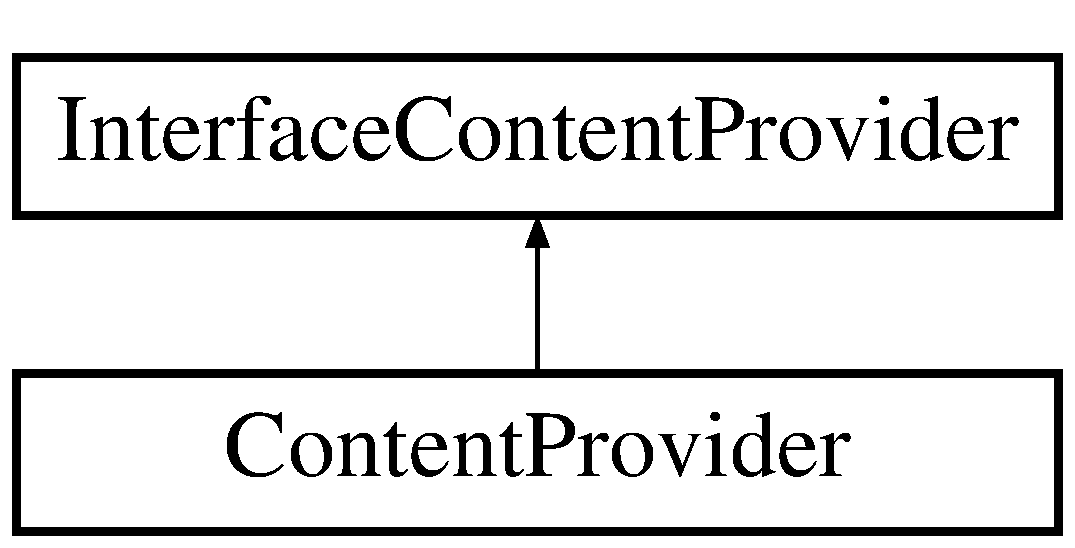
\includegraphics[height=2.000000cm]{class_david_fricker_1_1_data_abstracter_1_1_content_provider}
\end{center}
\end{figure}
\subsection*{Public Member Functions}
\begin{DoxyCompactItemize}
\item 
\hyperlink{class_david_fricker_1_1_data_abstracter_1_1_content_provider_a095c5d389db211932136b53f25f39685}{\+\_\+\+\_\+construct} ()
\end{DoxyCompactItemize}


\subsection{Constructor \& Destructor Documentation}
\mbox{\Hypertarget{class_david_fricker_1_1_data_abstracter_1_1_content_provider_a095c5d389db211932136b53f25f39685}\label{class_david_fricker_1_1_data_abstracter_1_1_content_provider_a095c5d389db211932136b53f25f39685}} 
\index{David\+Fricker\+::\+Data\+Abstracter\+::\+Content\+Provider@{David\+Fricker\+::\+Data\+Abstracter\+::\+Content\+Provider}!\+\_\+\+\_\+construct@{\+\_\+\+\_\+construct}}
\index{\+\_\+\+\_\+construct@{\+\_\+\+\_\+construct}!David\+Fricker\+::\+Data\+Abstracter\+::\+Content\+Provider@{David\+Fricker\+::\+Data\+Abstracter\+::\+Content\+Provider}}
\subsubsection{\texorpdfstring{\+\_\+\+\_\+construct()}{\_\_construct()}}
{\footnotesize\ttfamily \+\_\+\+\_\+construct (\begin{DoxyParamCaption}{ }\end{DoxyParamCaption})}



The documentation for this class was generated from the following file\+:\begin{DoxyCompactItemize}
\item 
D\+:/\+X\+A\+M\+P\+P/htdocs/\+Data\+Abstracter/src/\hyperlink{_content_provider_8php}{Content\+Provider.\+php}\end{DoxyCompactItemize}

\hypertarget{interface_david_fricker_1_1_data_abstracter_1_1_interface_content_provider}{}\section{Interface\+Content\+Provider Interface Reference}
\label{interface_david_fricker_1_1_data_abstracter_1_1_interface_content_provider}\index{Interface\+Content\+Provider@{Interface\+Content\+Provider}}
Inheritance diagram for Interface\+Content\+Provider\+:\begin{figure}[H]
\begin{center}
\leavevmode
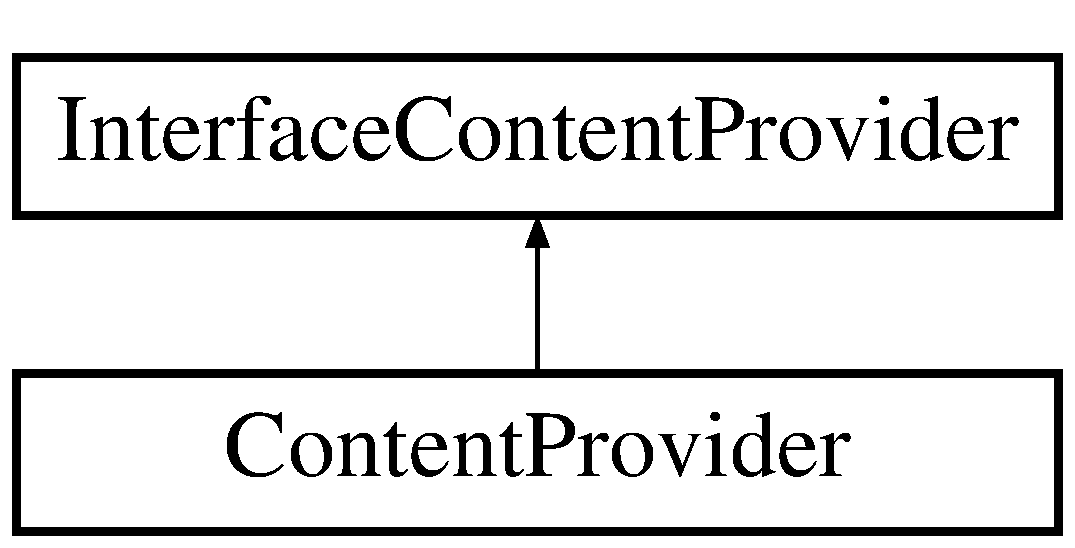
\includegraphics[height=2.000000cm]{interface_david_fricker_1_1_data_abstracter_1_1_interface_content_provider}
\end{center}
\end{figure}
\subsection*{Public Member Functions}
\begin{DoxyCompactItemize}
\item 
\hyperlink{interface_david_fricker_1_1_data_abstracter_1_1_interface_content_provider_ae08b1d097cd6b6e5982ef0e0fd71de26}{insert} (\$table, \$data)
\item 
\hyperlink{interface_david_fricker_1_1_data_abstracter_1_1_interface_content_provider_a2793579c78ddc2f9f2428185305ddc88}{delete} (\$table, \$where=false, \$limit=false)
\item 
\hyperlink{interface_david_fricker_1_1_data_abstracter_1_1_interface_content_provider_a085afde80e8bee8ebfa89775b4d1446f}{update} (\$table, \$data, \$where=false, \$limit=false)
\item 
\hyperlink{interface_david_fricker_1_1_data_abstracter_1_1_interface_content_provider_ab2ab0042470a76f29458dff737c7769f}{fetch} (\$table, \$columns, \$where=false, \$limit=false)
\item 
\hyperlink{interface_david_fricker_1_1_data_abstracter_1_1_interface_content_provider_ae0a8b5efb674b9222fe1a21014d078ea}{run} (\$query)
\end{DoxyCompactItemize}


\subsection{Member Function Documentation}
\mbox{\Hypertarget{interface_david_fricker_1_1_data_abstracter_1_1_interface_content_provider_a2793579c78ddc2f9f2428185305ddc88}\label{interface_david_fricker_1_1_data_abstracter_1_1_interface_content_provider_a2793579c78ddc2f9f2428185305ddc88}} 
\index{David\+Fricker\+::\+Data\+Abstracter\+::\+Interface\+Content\+Provider@{David\+Fricker\+::\+Data\+Abstracter\+::\+Interface\+Content\+Provider}!delete@{delete}}
\index{delete@{delete}!David\+Fricker\+::\+Data\+Abstracter\+::\+Interface\+Content\+Provider@{David\+Fricker\+::\+Data\+Abstracter\+::\+Interface\+Content\+Provider}}
\subsubsection{\texorpdfstring{delete()}{delete()}}
{\footnotesize\ttfamily delete (\begin{DoxyParamCaption}\item[{}]{\$table,  }\item[{}]{\$where = {\ttfamily false},  }\item[{}]{\$limit = {\ttfamily false} }\end{DoxyParamCaption})}

\mbox{\Hypertarget{interface_david_fricker_1_1_data_abstracter_1_1_interface_content_provider_ab2ab0042470a76f29458dff737c7769f}\label{interface_david_fricker_1_1_data_abstracter_1_1_interface_content_provider_ab2ab0042470a76f29458dff737c7769f}} 
\index{David\+Fricker\+::\+Data\+Abstracter\+::\+Interface\+Content\+Provider@{David\+Fricker\+::\+Data\+Abstracter\+::\+Interface\+Content\+Provider}!fetch@{fetch}}
\index{fetch@{fetch}!David\+Fricker\+::\+Data\+Abstracter\+::\+Interface\+Content\+Provider@{David\+Fricker\+::\+Data\+Abstracter\+::\+Interface\+Content\+Provider}}
\subsubsection{\texorpdfstring{fetch()}{fetch()}}
{\footnotesize\ttfamily fetch (\begin{DoxyParamCaption}\item[{}]{\$table,  }\item[{}]{\$columns,  }\item[{}]{\$where = {\ttfamily false},  }\item[{}]{\$limit = {\ttfamily false} }\end{DoxyParamCaption})}

\mbox{\Hypertarget{interface_david_fricker_1_1_data_abstracter_1_1_interface_content_provider_ae08b1d097cd6b6e5982ef0e0fd71de26}\label{interface_david_fricker_1_1_data_abstracter_1_1_interface_content_provider_ae08b1d097cd6b6e5982ef0e0fd71de26}} 
\index{David\+Fricker\+::\+Data\+Abstracter\+::\+Interface\+Content\+Provider@{David\+Fricker\+::\+Data\+Abstracter\+::\+Interface\+Content\+Provider}!insert@{insert}}
\index{insert@{insert}!David\+Fricker\+::\+Data\+Abstracter\+::\+Interface\+Content\+Provider@{David\+Fricker\+::\+Data\+Abstracter\+::\+Interface\+Content\+Provider}}
\subsubsection{\texorpdfstring{insert()}{insert()}}
{\footnotesize\ttfamily insert (\begin{DoxyParamCaption}\item[{}]{\$table,  }\item[{}]{\$data }\end{DoxyParamCaption})}

\mbox{\Hypertarget{interface_david_fricker_1_1_data_abstracter_1_1_interface_content_provider_ae0a8b5efb674b9222fe1a21014d078ea}\label{interface_david_fricker_1_1_data_abstracter_1_1_interface_content_provider_ae0a8b5efb674b9222fe1a21014d078ea}} 
\index{David\+Fricker\+::\+Data\+Abstracter\+::\+Interface\+Content\+Provider@{David\+Fricker\+::\+Data\+Abstracter\+::\+Interface\+Content\+Provider}!run@{run}}
\index{run@{run}!David\+Fricker\+::\+Data\+Abstracter\+::\+Interface\+Content\+Provider@{David\+Fricker\+::\+Data\+Abstracter\+::\+Interface\+Content\+Provider}}
\subsubsection{\texorpdfstring{run()}{run()}}
{\footnotesize\ttfamily run (\begin{DoxyParamCaption}\item[{}]{\$query }\end{DoxyParamCaption})}

\mbox{\Hypertarget{interface_david_fricker_1_1_data_abstracter_1_1_interface_content_provider_a085afde80e8bee8ebfa89775b4d1446f}\label{interface_david_fricker_1_1_data_abstracter_1_1_interface_content_provider_a085afde80e8bee8ebfa89775b4d1446f}} 
\index{David\+Fricker\+::\+Data\+Abstracter\+::\+Interface\+Content\+Provider@{David\+Fricker\+::\+Data\+Abstracter\+::\+Interface\+Content\+Provider}!update@{update}}
\index{update@{update}!David\+Fricker\+::\+Data\+Abstracter\+::\+Interface\+Content\+Provider@{David\+Fricker\+::\+Data\+Abstracter\+::\+Interface\+Content\+Provider}}
\subsubsection{\texorpdfstring{update()}{update()}}
{\footnotesize\ttfamily update (\begin{DoxyParamCaption}\item[{}]{\$table,  }\item[{}]{\$data,  }\item[{}]{\$where = {\ttfamily false},  }\item[{}]{\$limit = {\ttfamily false} }\end{DoxyParamCaption})}



The documentation for this interface was generated from the following file\+:\begin{DoxyCompactItemize}
\item 
D\+:/\+X\+A\+M\+P\+P/htdocs/\+Data\+Abstracter/src/\hyperlink{_interface_content_provider_8php}{Interface\+Content\+Provider.\+php}\end{DoxyCompactItemize}

\hypertarget{interface_david_fricker_1_1_data_abstracter_1_1_interface_database_wrapper}{}\section{Interface\+Database\+Wrapper Interface Reference}
\label{interface_david_fricker_1_1_data_abstracter_1_1_interface_database_wrapper}\index{Interface\+Database\+Wrapper@{Interface\+Database\+Wrapper}}
Inheritance diagram for Interface\+Database\+Wrapper\+:\begin{figure}[H]
\begin{center}
\leavevmode
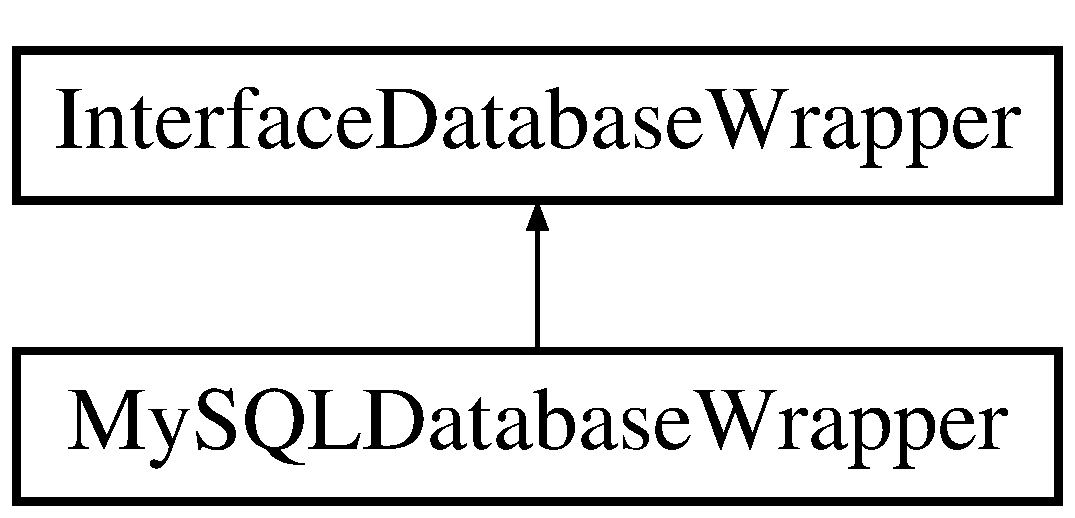
\includegraphics[height=2.000000cm]{interface_david_fricker_1_1_data_abstracter_1_1_interface_database_wrapper}
\end{center}
\end{figure}
\subsection*{Public Member Functions}
\begin{DoxyCompactItemize}
\item 
\hyperlink{interface_david_fricker_1_1_data_abstracter_1_1_interface_database_wrapper_ae08b1d097cd6b6e5982ef0e0fd71de26}{insert} (\$table, \$data)
\item 
\hyperlink{interface_david_fricker_1_1_data_abstracter_1_1_interface_database_wrapper_af5ba80c2cc9f719100a159c8044959c4}{delete} (\$table, \$where, \$limit)
\item 
\hyperlink{interface_david_fricker_1_1_data_abstracter_1_1_interface_database_wrapper_a01031130a0d4895f40ffe781941c7d9d}{update} (\$table, \$data, \$where, \$limit)
\item 
\hyperlink{interface_david_fricker_1_1_data_abstracter_1_1_interface_database_wrapper_a1c059eb42ed90b66113b3d72a2ce556b}{fetch} (\$table, \$columns, \$where, \$limit)
\item 
\hyperlink{interface_david_fricker_1_1_data_abstracter_1_1_interface_database_wrapper_ae0a8b5efb674b9222fe1a21014d078ea}{run} (\$query)
\end{DoxyCompactItemize}


\subsection{Member Function Documentation}
\mbox{\Hypertarget{interface_david_fricker_1_1_data_abstracter_1_1_interface_database_wrapper_af5ba80c2cc9f719100a159c8044959c4}\label{interface_david_fricker_1_1_data_abstracter_1_1_interface_database_wrapper_af5ba80c2cc9f719100a159c8044959c4}} 
\index{David\+Fricker\+::\+Data\+Abstracter\+::\+Interface\+Database\+Wrapper@{David\+Fricker\+::\+Data\+Abstracter\+::\+Interface\+Database\+Wrapper}!delete@{delete}}
\index{delete@{delete}!David\+Fricker\+::\+Data\+Abstracter\+::\+Interface\+Database\+Wrapper@{David\+Fricker\+::\+Data\+Abstracter\+::\+Interface\+Database\+Wrapper}}
\subsubsection{\texorpdfstring{delete()}{delete()}}
{\footnotesize\ttfamily delete (\begin{DoxyParamCaption}\item[{}]{\$table,  }\item[{}]{\$where,  }\item[{}]{\$limit }\end{DoxyParamCaption})}



Implemented in \hyperlink{class_david_fricker_1_1_data_abstracter_1_1_my_s_q_l_database_wrapper_af5ba80c2cc9f719100a159c8044959c4}{My\+S\+Q\+L\+Database\+Wrapper}.

\mbox{\Hypertarget{interface_david_fricker_1_1_data_abstracter_1_1_interface_database_wrapper_a1c059eb42ed90b66113b3d72a2ce556b}\label{interface_david_fricker_1_1_data_abstracter_1_1_interface_database_wrapper_a1c059eb42ed90b66113b3d72a2ce556b}} 
\index{David\+Fricker\+::\+Data\+Abstracter\+::\+Interface\+Database\+Wrapper@{David\+Fricker\+::\+Data\+Abstracter\+::\+Interface\+Database\+Wrapper}!fetch@{fetch}}
\index{fetch@{fetch}!David\+Fricker\+::\+Data\+Abstracter\+::\+Interface\+Database\+Wrapper@{David\+Fricker\+::\+Data\+Abstracter\+::\+Interface\+Database\+Wrapper}}
\subsubsection{\texorpdfstring{fetch()}{fetch()}}
{\footnotesize\ttfamily fetch (\begin{DoxyParamCaption}\item[{}]{\$table,  }\item[{}]{\$columns,  }\item[{}]{\$where,  }\item[{}]{\$limit }\end{DoxyParamCaption})}



Implemented in \hyperlink{class_david_fricker_1_1_data_abstracter_1_1_my_s_q_l_database_wrapper_ab2ab0042470a76f29458dff737c7769f}{My\+S\+Q\+L\+Database\+Wrapper}.

\mbox{\Hypertarget{interface_david_fricker_1_1_data_abstracter_1_1_interface_database_wrapper_ae08b1d097cd6b6e5982ef0e0fd71de26}\label{interface_david_fricker_1_1_data_abstracter_1_1_interface_database_wrapper_ae08b1d097cd6b6e5982ef0e0fd71de26}} 
\index{David\+Fricker\+::\+Data\+Abstracter\+::\+Interface\+Database\+Wrapper@{David\+Fricker\+::\+Data\+Abstracter\+::\+Interface\+Database\+Wrapper}!insert@{insert}}
\index{insert@{insert}!David\+Fricker\+::\+Data\+Abstracter\+::\+Interface\+Database\+Wrapper@{David\+Fricker\+::\+Data\+Abstracter\+::\+Interface\+Database\+Wrapper}}
\subsubsection{\texorpdfstring{insert()}{insert()}}
{\footnotesize\ttfamily insert (\begin{DoxyParamCaption}\item[{}]{\$table,  }\item[{}]{\$data }\end{DoxyParamCaption})}



Implemented in \hyperlink{class_david_fricker_1_1_data_abstracter_1_1_my_s_q_l_database_wrapper_ae08b1d097cd6b6e5982ef0e0fd71de26}{My\+S\+Q\+L\+Database\+Wrapper}.

\mbox{\Hypertarget{interface_david_fricker_1_1_data_abstracter_1_1_interface_database_wrapper_ae0a8b5efb674b9222fe1a21014d078ea}\label{interface_david_fricker_1_1_data_abstracter_1_1_interface_database_wrapper_ae0a8b5efb674b9222fe1a21014d078ea}} 
\index{David\+Fricker\+::\+Data\+Abstracter\+::\+Interface\+Database\+Wrapper@{David\+Fricker\+::\+Data\+Abstracter\+::\+Interface\+Database\+Wrapper}!run@{run}}
\index{run@{run}!David\+Fricker\+::\+Data\+Abstracter\+::\+Interface\+Database\+Wrapper@{David\+Fricker\+::\+Data\+Abstracter\+::\+Interface\+Database\+Wrapper}}
\subsubsection{\texorpdfstring{run()}{run()}}
{\footnotesize\ttfamily run (\begin{DoxyParamCaption}\item[{}]{\$query }\end{DoxyParamCaption})}

\mbox{\Hypertarget{interface_david_fricker_1_1_data_abstracter_1_1_interface_database_wrapper_a01031130a0d4895f40ffe781941c7d9d}\label{interface_david_fricker_1_1_data_abstracter_1_1_interface_database_wrapper_a01031130a0d4895f40ffe781941c7d9d}} 
\index{David\+Fricker\+::\+Data\+Abstracter\+::\+Interface\+Database\+Wrapper@{David\+Fricker\+::\+Data\+Abstracter\+::\+Interface\+Database\+Wrapper}!update@{update}}
\index{update@{update}!David\+Fricker\+::\+Data\+Abstracter\+::\+Interface\+Database\+Wrapper@{David\+Fricker\+::\+Data\+Abstracter\+::\+Interface\+Database\+Wrapper}}
\subsubsection{\texorpdfstring{update()}{update()}}
{\footnotesize\ttfamily update (\begin{DoxyParamCaption}\item[{}]{\$table,  }\item[{}]{\$data,  }\item[{}]{\$where,  }\item[{}]{\$limit }\end{DoxyParamCaption})}



Implemented in \hyperlink{class_david_fricker_1_1_data_abstracter_1_1_my_s_q_l_database_wrapper_a7fb294063cf3c7db8953cf241630d382}{My\+S\+Q\+L\+Database\+Wrapper}.



The documentation for this interface was generated from the following file\+:\begin{DoxyCompactItemize}
\item 
D\+:/\+X\+A\+M\+P\+P/htdocs/\+Data\+Abstracter/src/\hyperlink{_interface_database_wrapper_8php}{Interface\+Database\+Wrapper.\+php}\end{DoxyCompactItemize}

\hypertarget{class_david_fricker_1_1_data_abstracter_1_1_my_s_q_l_database_wrapper}{}\section{My\+S\+Q\+L\+Database\+Wrapper Class Reference}
\label{class_david_fricker_1_1_data_abstracter_1_1_my_s_q_l_database_wrapper}\index{My\+S\+Q\+L\+Database\+Wrapper@{My\+S\+Q\+L\+Database\+Wrapper}}
Inheritance diagram for My\+S\+Q\+L\+Database\+Wrapper\+:\begin{figure}[H]
\begin{center}
\leavevmode
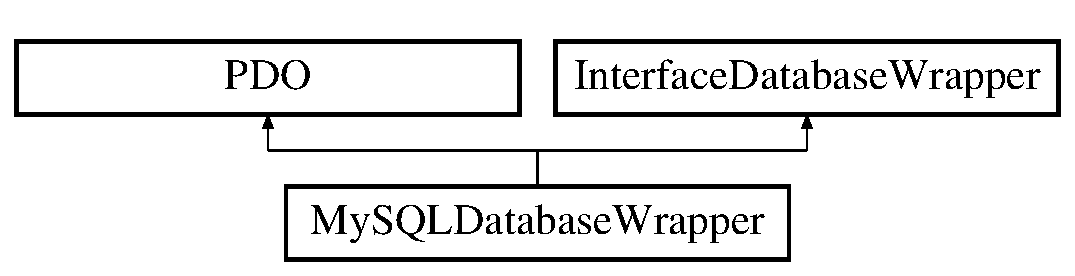
\includegraphics[height=2.000000cm]{class_david_fricker_1_1_data_abstracter_1_1_my_s_q_l_database_wrapper}
\end{center}
\end{figure}
\subsection*{Public Member Functions}
\begin{DoxyCompactItemize}
\item 
\hyperlink{class_david_fricker_1_1_data_abstracter_1_1_my_s_q_l_database_wrapper_a095c5d389db211932136b53f25f39685}{\+\_\+\+\_\+construct} ()
\item 
\hyperlink{class_david_fricker_1_1_data_abstracter_1_1_my_s_q_l_database_wrapper_af5ba80c2cc9f719100a159c8044959c4}{delete} (\$table, \$where, \$limit)
\item 
\hyperlink{class_david_fricker_1_1_data_abstracter_1_1_my_s_q_l_database_wrapper_a7fb294063cf3c7db8953cf241630d382}{update} (\$table, \$data, \$where, \$limit=false)
\item 
\hyperlink{class_david_fricker_1_1_data_abstracter_1_1_my_s_q_l_database_wrapper_ab2ab0042470a76f29458dff737c7769f}{fetch} (\$table, \$columns, \$where=false, \$limit=false)
\item 
\hyperlink{class_david_fricker_1_1_data_abstracter_1_1_my_s_q_l_database_wrapper_ae08b1d097cd6b6e5982ef0e0fd71de26}{insert} (\$table, \$data)
\item 
\hyperlink{class_david_fricker_1_1_data_abstracter_1_1_my_s_q_l_database_wrapper_ae568f0a5e65e08bb6de8e728846ad0c0}{run} (\$query, \$bind=\mbox{[}$\,$\mbox{]})
\item 
\hyperlink{class_david_fricker_1_1_data_abstracter_1_1_my_s_q_l_database_wrapper_afd1c56cdadff97f9d86095f745e95658}{get\+Last\+Insert\+ID} ()
\item 
\hyperlink{class_david_fricker_1_1_data_abstracter_1_1_my_s_q_l_database_wrapper_a82b073888555fc72e57142fe913db377}{row\+Count} ()
\item 
\hyperlink{class_david_fricker_1_1_data_abstracter_1_1_my_s_q_l_database_wrapper_a03582271ad4fdc21fa01a7901bf3605f}{get\+Last\+Error} ()
\item 
\hyperlink{class_david_fricker_1_1_data_abstracter_1_1_my_s_q_l_database_wrapper_aec4449be5da742126a819826b02be73b}{is\+Valid\+Column} (\$table, \$column)
\end{DoxyCompactItemize}


\subsection{Constructor \& Destructor Documentation}
\mbox{\Hypertarget{class_david_fricker_1_1_data_abstracter_1_1_my_s_q_l_database_wrapper_a095c5d389db211932136b53f25f39685}\label{class_david_fricker_1_1_data_abstracter_1_1_my_s_q_l_database_wrapper_a095c5d389db211932136b53f25f39685}} 
\index{David\+Fricker\+::\+Data\+Abstracter\+::\+My\+S\+Q\+L\+Database\+Wrapper@{David\+Fricker\+::\+Data\+Abstracter\+::\+My\+S\+Q\+L\+Database\+Wrapper}!\+\_\+\+\_\+construct@{\+\_\+\+\_\+construct}}
\index{\+\_\+\+\_\+construct@{\+\_\+\+\_\+construct}!David\+Fricker\+::\+Data\+Abstracter\+::\+My\+S\+Q\+L\+Database\+Wrapper@{David\+Fricker\+::\+Data\+Abstracter\+::\+My\+S\+Q\+L\+Database\+Wrapper}}
\subsubsection{\texorpdfstring{\+\_\+\+\_\+construct()}{\_\_construct()}}
{\footnotesize\ttfamily \+\_\+\+\_\+construct (\begin{DoxyParamCaption}{ }\end{DoxyParamCaption})}



\subsection{Member Function Documentation}
\mbox{\Hypertarget{class_david_fricker_1_1_data_abstracter_1_1_my_s_q_l_database_wrapper_af5ba80c2cc9f719100a159c8044959c4}\label{class_david_fricker_1_1_data_abstracter_1_1_my_s_q_l_database_wrapper_af5ba80c2cc9f719100a159c8044959c4}} 
\index{David\+Fricker\+::\+Data\+Abstracter\+::\+My\+S\+Q\+L\+Database\+Wrapper@{David\+Fricker\+::\+Data\+Abstracter\+::\+My\+S\+Q\+L\+Database\+Wrapper}!delete@{delete}}
\index{delete@{delete}!David\+Fricker\+::\+Data\+Abstracter\+::\+My\+S\+Q\+L\+Database\+Wrapper@{David\+Fricker\+::\+Data\+Abstracter\+::\+My\+S\+Q\+L\+Database\+Wrapper}}
\subsubsection{\texorpdfstring{delete()}{delete()}}
{\footnotesize\ttfamily delete (\begin{DoxyParamCaption}\item[{}]{\$table,  }\item[{}]{\$where,  }\item[{}]{\$limit }\end{DoxyParamCaption})}



Implements \hyperlink{interface_david_fricker_1_1_data_abstracter_1_1_interface_database_wrapper_af5ba80c2cc9f719100a159c8044959c4}{Interface\+Database\+Wrapper}.

\mbox{\Hypertarget{class_david_fricker_1_1_data_abstracter_1_1_my_s_q_l_database_wrapper_ab2ab0042470a76f29458dff737c7769f}\label{class_david_fricker_1_1_data_abstracter_1_1_my_s_q_l_database_wrapper_ab2ab0042470a76f29458dff737c7769f}} 
\index{David\+Fricker\+::\+Data\+Abstracter\+::\+My\+S\+Q\+L\+Database\+Wrapper@{David\+Fricker\+::\+Data\+Abstracter\+::\+My\+S\+Q\+L\+Database\+Wrapper}!fetch@{fetch}}
\index{fetch@{fetch}!David\+Fricker\+::\+Data\+Abstracter\+::\+My\+S\+Q\+L\+Database\+Wrapper@{David\+Fricker\+::\+Data\+Abstracter\+::\+My\+S\+Q\+L\+Database\+Wrapper}}
\subsubsection{\texorpdfstring{fetch()}{fetch()}}
{\footnotesize\ttfamily fetch (\begin{DoxyParamCaption}\item[{}]{\$table,  }\item[{}]{\$columns,  }\item[{}]{\$where = {\ttfamily false},  }\item[{}]{\$limit = {\ttfamily false} }\end{DoxyParamCaption})}



Implements \hyperlink{interface_david_fricker_1_1_data_abstracter_1_1_interface_database_wrapper_a1c059eb42ed90b66113b3d72a2ce556b}{Interface\+Database\+Wrapper}.

\mbox{\Hypertarget{class_david_fricker_1_1_data_abstracter_1_1_my_s_q_l_database_wrapper_a03582271ad4fdc21fa01a7901bf3605f}\label{class_david_fricker_1_1_data_abstracter_1_1_my_s_q_l_database_wrapper_a03582271ad4fdc21fa01a7901bf3605f}} 
\index{David\+Fricker\+::\+Data\+Abstracter\+::\+My\+S\+Q\+L\+Database\+Wrapper@{David\+Fricker\+::\+Data\+Abstracter\+::\+My\+S\+Q\+L\+Database\+Wrapper}!get\+Last\+Error@{get\+Last\+Error}}
\index{get\+Last\+Error@{get\+Last\+Error}!David\+Fricker\+::\+Data\+Abstracter\+::\+My\+S\+Q\+L\+Database\+Wrapper@{David\+Fricker\+::\+Data\+Abstracter\+::\+My\+S\+Q\+L\+Database\+Wrapper}}
\subsubsection{\texorpdfstring{get\+Last\+Error()}{getLastError()}}
{\footnotesize\ttfamily get\+Last\+Error (\begin{DoxyParamCaption}{ }\end{DoxyParamCaption})}

\mbox{\Hypertarget{class_david_fricker_1_1_data_abstracter_1_1_my_s_q_l_database_wrapper_afd1c56cdadff97f9d86095f745e95658}\label{class_david_fricker_1_1_data_abstracter_1_1_my_s_q_l_database_wrapper_afd1c56cdadff97f9d86095f745e95658}} 
\index{David\+Fricker\+::\+Data\+Abstracter\+::\+My\+S\+Q\+L\+Database\+Wrapper@{David\+Fricker\+::\+Data\+Abstracter\+::\+My\+S\+Q\+L\+Database\+Wrapper}!get\+Last\+Insert\+ID@{get\+Last\+Insert\+ID}}
\index{get\+Last\+Insert\+ID@{get\+Last\+Insert\+ID}!David\+Fricker\+::\+Data\+Abstracter\+::\+My\+S\+Q\+L\+Database\+Wrapper@{David\+Fricker\+::\+Data\+Abstracter\+::\+My\+S\+Q\+L\+Database\+Wrapper}}
\subsubsection{\texorpdfstring{get\+Last\+Insert\+I\+D()}{getLastInsertID()}}
{\footnotesize\ttfamily get\+Last\+Insert\+ID (\begin{DoxyParamCaption}{ }\end{DoxyParamCaption})}

\mbox{\Hypertarget{class_david_fricker_1_1_data_abstracter_1_1_my_s_q_l_database_wrapper_ae08b1d097cd6b6e5982ef0e0fd71de26}\label{class_david_fricker_1_1_data_abstracter_1_1_my_s_q_l_database_wrapper_ae08b1d097cd6b6e5982ef0e0fd71de26}} 
\index{David\+Fricker\+::\+Data\+Abstracter\+::\+My\+S\+Q\+L\+Database\+Wrapper@{David\+Fricker\+::\+Data\+Abstracter\+::\+My\+S\+Q\+L\+Database\+Wrapper}!insert@{insert}}
\index{insert@{insert}!David\+Fricker\+::\+Data\+Abstracter\+::\+My\+S\+Q\+L\+Database\+Wrapper@{David\+Fricker\+::\+Data\+Abstracter\+::\+My\+S\+Q\+L\+Database\+Wrapper}}
\subsubsection{\texorpdfstring{insert()}{insert()}}
{\footnotesize\ttfamily insert (\begin{DoxyParamCaption}\item[{}]{\$table,  }\item[{}]{\$data }\end{DoxyParamCaption})}



Implements \hyperlink{interface_david_fricker_1_1_data_abstracter_1_1_interface_database_wrapper_ae08b1d097cd6b6e5982ef0e0fd71de26}{Interface\+Database\+Wrapper}.

\mbox{\Hypertarget{class_david_fricker_1_1_data_abstracter_1_1_my_s_q_l_database_wrapper_aec4449be5da742126a819826b02be73b}\label{class_david_fricker_1_1_data_abstracter_1_1_my_s_q_l_database_wrapper_aec4449be5da742126a819826b02be73b}} 
\index{David\+Fricker\+::\+Data\+Abstracter\+::\+My\+S\+Q\+L\+Database\+Wrapper@{David\+Fricker\+::\+Data\+Abstracter\+::\+My\+S\+Q\+L\+Database\+Wrapper}!is\+Valid\+Column@{is\+Valid\+Column}}
\index{is\+Valid\+Column@{is\+Valid\+Column}!David\+Fricker\+::\+Data\+Abstracter\+::\+My\+S\+Q\+L\+Database\+Wrapper@{David\+Fricker\+::\+Data\+Abstracter\+::\+My\+S\+Q\+L\+Database\+Wrapper}}
\subsubsection{\texorpdfstring{is\+Valid\+Column()}{isValidColumn()}}
{\footnotesize\ttfamily is\+Valid\+Column (\begin{DoxyParamCaption}\item[{}]{\$table,  }\item[{}]{\$column }\end{DoxyParamCaption})}

\mbox{\Hypertarget{class_david_fricker_1_1_data_abstracter_1_1_my_s_q_l_database_wrapper_a82b073888555fc72e57142fe913db377}\label{class_david_fricker_1_1_data_abstracter_1_1_my_s_q_l_database_wrapper_a82b073888555fc72e57142fe913db377}} 
\index{David\+Fricker\+::\+Data\+Abstracter\+::\+My\+S\+Q\+L\+Database\+Wrapper@{David\+Fricker\+::\+Data\+Abstracter\+::\+My\+S\+Q\+L\+Database\+Wrapper}!row\+Count@{row\+Count}}
\index{row\+Count@{row\+Count}!David\+Fricker\+::\+Data\+Abstracter\+::\+My\+S\+Q\+L\+Database\+Wrapper@{David\+Fricker\+::\+Data\+Abstracter\+::\+My\+S\+Q\+L\+Database\+Wrapper}}
\subsubsection{\texorpdfstring{row\+Count()}{rowCount()}}
{\footnotesize\ttfamily row\+Count (\begin{DoxyParamCaption}{ }\end{DoxyParamCaption})}

\mbox{\Hypertarget{class_david_fricker_1_1_data_abstracter_1_1_my_s_q_l_database_wrapper_ae568f0a5e65e08bb6de8e728846ad0c0}\label{class_david_fricker_1_1_data_abstracter_1_1_my_s_q_l_database_wrapper_ae568f0a5e65e08bb6de8e728846ad0c0}} 
\index{David\+Fricker\+::\+Data\+Abstracter\+::\+My\+S\+Q\+L\+Database\+Wrapper@{David\+Fricker\+::\+Data\+Abstracter\+::\+My\+S\+Q\+L\+Database\+Wrapper}!run@{run}}
\index{run@{run}!David\+Fricker\+::\+Data\+Abstracter\+::\+My\+S\+Q\+L\+Database\+Wrapper@{David\+Fricker\+::\+Data\+Abstracter\+::\+My\+S\+Q\+L\+Database\+Wrapper}}
\subsubsection{\texorpdfstring{run()}{run()}}
{\footnotesize\ttfamily run (\begin{DoxyParamCaption}\item[{}]{\$query,  }\item[{}]{\$bind = {\ttfamily \mbox{[}\mbox{]}} }\end{DoxyParamCaption})}

\mbox{\Hypertarget{class_david_fricker_1_1_data_abstracter_1_1_my_s_q_l_database_wrapper_a7fb294063cf3c7db8953cf241630d382}\label{class_david_fricker_1_1_data_abstracter_1_1_my_s_q_l_database_wrapper_a7fb294063cf3c7db8953cf241630d382}} 
\index{David\+Fricker\+::\+Data\+Abstracter\+::\+My\+S\+Q\+L\+Database\+Wrapper@{David\+Fricker\+::\+Data\+Abstracter\+::\+My\+S\+Q\+L\+Database\+Wrapper}!update@{update}}
\index{update@{update}!David\+Fricker\+::\+Data\+Abstracter\+::\+My\+S\+Q\+L\+Database\+Wrapper@{David\+Fricker\+::\+Data\+Abstracter\+::\+My\+S\+Q\+L\+Database\+Wrapper}}
\subsubsection{\texorpdfstring{update()}{update()}}
{\footnotesize\ttfamily update (\begin{DoxyParamCaption}\item[{}]{\$table,  }\item[{}]{\$data,  }\item[{}]{\$where,  }\item[{}]{\$limit = {\ttfamily false} }\end{DoxyParamCaption})}



Implements \hyperlink{interface_david_fricker_1_1_data_abstracter_1_1_interface_database_wrapper_a01031130a0d4895f40ffe781941c7d9d}{Interface\+Database\+Wrapper}.



The documentation for this class was generated from the following file\+:\begin{DoxyCompactItemize}
\item 
D\+:/\+X\+A\+M\+P\+P/htdocs/\+Data\+Abstracter/src/\hyperlink{_my_s_q_l_database_wrapper_8php}{My\+S\+Q\+L\+Database\+Wrapper.\+php}\end{DoxyCompactItemize}

\chapter{File Documentation}
\hypertarget{_content_contract_8php}{}\section{D\+:/\+X\+A\+M\+P\+P/htdocs/\+Data\+Abstracter/src/\+Content\+Contract.php File Reference}
\label{_content_contract_8php}\index{D\+:/\+X\+A\+M\+P\+P/htdocs/\+Data\+Abstracter/src/\+Content\+Contract.\+php@{D\+:/\+X\+A\+M\+P\+P/htdocs/\+Data\+Abstracter/src/\+Content\+Contract.\+php}}
\subsection*{Data Structures}
\begin{DoxyCompactItemize}
\item 
class \hyperlink{class_david_fricker_1_1_data_abstracter_1_1_content_contract}{Content\+Contract}
\end{DoxyCompactItemize}
\subsection*{Namespaces}
\begin{DoxyCompactItemize}
\item 
 \hyperlink{namespace_david_fricker_1_1_data_abstracter}{David\+Fricker\textbackslash{}\+Data\+Abstracter}
\end{DoxyCompactItemize}

\hypertarget{_content_provider_8php}{}\section{D\+:/\+X\+A\+M\+P\+P/htdocs/\+Data\+Abstracter/src/\+Content\+Provider.php File Reference}
\label{_content_provider_8php}\index{D\+:/\+X\+A\+M\+P\+P/htdocs/\+Data\+Abstracter/src/\+Content\+Provider.\+php@{D\+:/\+X\+A\+M\+P\+P/htdocs/\+Data\+Abstracter/src/\+Content\+Provider.\+php}}
\subsection*{Data Structures}
\begin{DoxyCompactItemize}
\item 
class \hyperlink{class_david_fricker_1_1_data_abstracter_1_1_content_provider}{Content\+Provider}
\end{DoxyCompactItemize}
\subsection*{Namespaces}
\begin{DoxyCompactItemize}
\item 
 \hyperlink{namespace_david_fricker_1_1_data_abstracter}{David\+Fricker\textbackslash{}\+Data\+Abstracter}
\end{DoxyCompactItemize}

\hypertarget{_interface_content_provider_8php}{}\section{D\+:/\+X\+A\+M\+P\+P/htdocs/\+Data\+Abstracter/src/\+Interface\+Content\+Provider.php File Reference}
\label{_interface_content_provider_8php}\index{D\+:/\+X\+A\+M\+P\+P/htdocs/\+Data\+Abstracter/src/\+Interface\+Content\+Provider.\+php@{D\+:/\+X\+A\+M\+P\+P/htdocs/\+Data\+Abstracter/src/\+Interface\+Content\+Provider.\+php}}
\subsection*{Data Structures}
\begin{DoxyCompactItemize}
\item 
interface \hyperlink{interface_david_fricker_1_1_data_abstracter_1_1_interface_content_provider}{Interface\+Content\+Provider}
\end{DoxyCompactItemize}
\subsection*{Namespaces}
\begin{DoxyCompactItemize}
\item 
 \hyperlink{namespace_david_fricker_1_1_data_abstracter}{David\+Fricker\textbackslash{}\+Data\+Abstracter}
\end{DoxyCompactItemize}

\hypertarget{_interface_database_wrapper_8php}{}\section{D\+:/\+X\+A\+M\+P\+P/htdocs/\+Data\+Abstracter/src/\+Interface\+Database\+Wrapper.php File Reference}
\label{_interface_database_wrapper_8php}\index{D\+:/\+X\+A\+M\+P\+P/htdocs/\+Data\+Abstracter/src/\+Interface\+Database\+Wrapper.\+php@{D\+:/\+X\+A\+M\+P\+P/htdocs/\+Data\+Abstracter/src/\+Interface\+Database\+Wrapper.\+php}}
\subsection*{Data Structures}
\begin{DoxyCompactItemize}
\item 
interface \hyperlink{interface_david_fricker_1_1_data_abstracter_1_1_interface_database_wrapper}{Interface\+Database\+Wrapper}
\end{DoxyCompactItemize}
\subsection*{Namespaces}
\begin{DoxyCompactItemize}
\item 
 \hyperlink{namespace_david_fricker_1_1_data_abstracter}{David\+Fricker\textbackslash{}\+Data\+Abstracter}
\end{DoxyCompactItemize}

\hypertarget{_my_s_q_l_database_wrapper_8php}{}\section{D\+:/\+X\+A\+M\+P\+P/htdocs/\+Data\+Abstracter/src/\+My\+S\+Q\+L\+Database\+Wrapper.php File Reference}
\label{_my_s_q_l_database_wrapper_8php}\index{D\+:/\+X\+A\+M\+P\+P/htdocs/\+Data\+Abstracter/src/\+My\+S\+Q\+L\+Database\+Wrapper.\+php@{D\+:/\+X\+A\+M\+P\+P/htdocs/\+Data\+Abstracter/src/\+My\+S\+Q\+L\+Database\+Wrapper.\+php}}
\subsection*{Data Structures}
\begin{DoxyCompactItemize}
\item 
class \hyperlink{class_david_fricker_1_1_data_abstracter_1_1_my_s_q_l_database_wrapper}{My\+S\+Q\+L\+Database\+Wrapper}
\end{DoxyCompactItemize}
\subsection*{Namespaces}
\begin{DoxyCompactItemize}
\item 
 \hyperlink{namespace_david_fricker_1_1_data_abstracter}{David\+Fricker\textbackslash{}\+Data\+Abstracter}
\end{DoxyCompactItemize}

\hypertarget{test_8php}{}\section{D\+:/\+X\+A\+M\+P\+P/htdocs/\+Data\+Abstracter/src/test.php File Reference}
\label{test_8php}\index{D\+:/\+X\+A\+M\+P\+P/htdocs/\+Data\+Abstracter/src/test.\+php@{D\+:/\+X\+A\+M\+P\+P/htdocs/\+Data\+Abstracter/src/test.\+php}}
\subsection*{Variables}
\begin{DoxyCompactItemize}
\item 
\hyperlink{test_8php_ad52817a5e6420efa40ae5fdd053e4d5e}{\$\+D\+B\+Wrapper} = new \hyperlink{class_david_fricker_1_1_data_abstracter_1_1_my_s_q_l_database_wrapper}{My\+S\+Q\+L\+Database\+Wrapper}()
\item 
\hyperlink{test_8php_a112ef069ddc0454086e3d1e6d8d55d07}{\$result}
\end{DoxyCompactItemize}


\subsection{Variable Documentation}
\mbox{\Hypertarget{test_8php_ad52817a5e6420efa40ae5fdd053e4d5e}\label{test_8php_ad52817a5e6420efa40ae5fdd053e4d5e}} 
\index{test.\+php@{test.\+php}!\$\+D\+B\+Wrapper@{\$\+D\+B\+Wrapper}}
\index{\$\+D\+B\+Wrapper@{\$\+D\+B\+Wrapper}!test.\+php@{test.\+php}}
\subsubsection{\texorpdfstring{\$\+D\+B\+Wrapper}{$DBWrapper}}
{\footnotesize\ttfamily \$D\+B\+Wrapper = new \hyperlink{class_david_fricker_1_1_data_abstracter_1_1_my_s_q_l_database_wrapper}{My\+S\+Q\+L\+Database\+Wrapper}()}

\mbox{\Hypertarget{test_8php_a112ef069ddc0454086e3d1e6d8d55d07}\label{test_8php_a112ef069ddc0454086e3d1e6d8d55d07}} 
\index{test.\+php@{test.\+php}!\$result@{\$result}}
\index{\$result@{\$result}!test.\+php@{test.\+php}}
\subsubsection{\texorpdfstring{\$result}{$result}}
{\footnotesize\ttfamily \$result}

{\bfseries Initial value\+:}
\begin{DoxyCode}
= \hyperlink{test_8php_ad52817a5e6420efa40ae5fdd053e4d5e}{$DBWrapper}->fetch(
    ContentContract::TABLE[\textcolor{stringliteral}{'customers'}], 
    \textcolor{stringliteral}{'Email'},
    \textcolor{keyword}{false},
    5)
\end{DoxyCode}

%--- End generated contents ---

% Index
\backmatter
\newpage
\phantomsection
\clearemptydoublepage
\addcontentsline{toc}{chapter}{Index}
\printindex

\end{document}
